\documentclass[letterpaper,10pt]{article}
\usepackage[letterpaper, hmargin=1.8cm, vmargin = 2.5cm]{geometry} %Sets the page geometry
\usepackage{url}
\usepackage{hyperref}
\usepackage{multicol}
\usepackage[english]{babel}
\usepackage{setspace}
\setlength{\parskip}{1em} % Set space when paragraphs are used
\setlength{\parindent}{0in}

\usepackage{xcolor}
\usepackage{multicol}
\usepackage{float}
\usepackage{graphicx} % Package for \includegraphics
\usepackage{wrapfig} % Figure wrapping
\usepackage[T1]{fontenc} % Output font encoding for international characters
\usepackage{amssymb}
\usepackage{amsmath}
\numberwithin{equation}{section}

\usepackage{amsthm}
\usepackage{mathtools}
\usepackage{thmtools}
\usepackage{bbm}
\usepackage[autostyle]{csquotes}
\usepackage{doi}
\usepackage[
    backend=biber,
    style=authoryear-comp,
    natbib=true,
    sortlocale=en_US,
    url=false, 
    doi=true,
    eprint=false
]{biblatex}

\addbibresource{bibliography.bib}

\declaretheoremstyle[
    spaceabove=10pt, spacebelow=10pt,
    postheadspace=\newline
    ]{mystyle}
\declaretheoremstyle[    
    spaceabove=6pt, spacebelow=6pt,
    postheadspace=\newline,
    qed=\qedsymbol
    ]{mystyle_pf}

\declaretheorem[style=mystyle, thmbox=M]{theorem}
\numberwithin{theorem}{section}
\declaretheorem[style=mystyle, thmbox=M, numberlike=theorem]{lemma, proposition, corollary}
\declaretheorem[style=mystyle, thmbox=M]{remark}
\numberwithin{remark}{section}
\declaretheorem[style=mystyle, thmbox=M]{definition}
\declaretheorem[style=mystyle, thmbox=M]{assumption}
\declaretheorem[style=mystyle, thmbox=M]{example}
\numberwithin{example}{section}
\declaretheorem[style=mystyle_pf, thmbox=M]{proof}


% Other
\newtheorem{thm}{Theorem}
\newtheorem{lem}{Lemma}
\newtheorem{cor}{Corollary}
\newtheorem{prop}{Proposition}
\newtheorem{asm}{Assumption}
\newcommand{\calC}{\mathcal{C}}
\theoremstyle{definition}
\newtheorem{rem}{Remark}
\newtheorem{ex}{Example}
\newcommand{\UT}{\mathbb{U}_T}

\newcommand{\sumi}{\sum_{i=1}^n}
\newcommand{\calE}{\mathcal{E}}
\makeatother
\renewcommand{\hat}{\widehat}
\newcommand{\sumij}{\sum_{1\le i<j\le n}}
\newcommand{\E}{\mathbb{E}}
\newcommand{\1}{\mathbb{1}}
\newcommand{\Var}{\text{Var}}
\newcommand{\Cov}{\text{Cov}}
\newcommand{\calD}{\mathcal{D}}
\newcommand{\calX}{\mathcal{X}}
\renewcommand{\P}{\mathbbm{P}}

\DeclarePairedDelimiter\floor{\lfloor}{\rfloor} %Floor function
\DeclarePairedDelimiter\ceil{\lceil}{\rceil} %Ceil function
\DeclareMathOperator*{\argmax}{arg\,max} % argmax
\DeclareMathOperator*{\argmin}{arg\,min} % argmin
\newcommand{\indep}{\perp\!\!\!\!\perp} 


\begin{document}
\singlespacing
\title{Pointwise and Uniform Inference for the Two-Scale\\ Distributional Nearest Neighbor Estimator}
\date{Last edited: \today}
\author{Jakob R. Juergens \\ University of Wisconsin - Madison}
\maketitle
\hrule
\onehalfspacing
\begin{abstract}
	Recent advances in the literature on non-parametric regression and uniform inference for incomplete infinite-order U-statistics have enabled us to consider the problem of uniform inference for a broader class of estimators.
	One class of such estimators are bagged nearest neighbor estimators and among them specifically the Two-Scale Distributional Nearest Neighbor Estimator (TDNN) of \citet{demirkaya_optimal_2024}.
	In this paper, we develop uniform inference procedures based on recent work by \citet{ritzwoller_uniform_2024} for the TDNN estimator.
	As part of this work, we provide a complementary R package called \textit{tdnnR} that implements the presented methods.
\end{abstract}
\vspace{0.3cm}
\hrule
\singlespacing

\vspace{-0.3cm}
\begin{center}
	{\small Supplementary Material and R Package available at: \url{https://github.com/JakobJuergens/Unif_Inf_TDNN}}
\end{center}
\vspace{0.3cm}
\hrule
\singlespacing
% {\small \tableofcontents}
\thispagestyle{empty}

\pagenumbering{arabic}

\newpage
\onehalfspacing
\section{Introduction}
\hrule
Nearest Neighbor Estimators and their derivatives form a flexible class of estimators for a variety of purposes including nonparametric regression.
Although widely used in practice for the latter purpose, some of their properties are still elusive when it comes to performing inference.
This paper contributes to improving our understanding by establishing an asymptotically valid method to construct uniform confidence bands when using the Two-Scale Distributional Nearest Neighbor (TDNN) method of \citet{demirkaya_optimal_2024}.
To achieve this goal, we use novel results on uniform inference for infinite-order U-statistics (IOUS) developed in \citet{ritzwoller_uniform_2024}.
Due to the inherent connection of the Potential Nearest Neighbors (PNN) framework to Random Forests (RF), this work also contributes to contextualizing recent advances in inference techniques for random forests.
	{\color{red} LOREM IPSUM}

The remainder of this paper is organized as follows.
Section \ref{TDNN} introduces the TDNN estimator as developed by \citet{demirkaya_optimal_2024} and presents some of the results this paper is based on.
Section \ref{Subsampling_Improvements} uses recent theoretical developments to show that the distributional approximations provided by \citet{demirkaya_optimal_2024} can be justified under weaker assumptions on the chosen subsampling scales.
Section \ref{UnifInf} extends results from \citet{ritzwoller_uniform_2024} to the TDNN estimator and thus introduces methods to construct uniform confidence bands for the TDNN estimator.
Section \ref{Simulations} explores the performance of the developed uniform inference methods in a number of setups and Section \ref{Application} applies them to the context of {\color{red} LOREM IPSUM}.
Section \ref{Conclusion} concludes.

\subsection{Notation}
\begin{itemize}
	\item $\rightsquigarrow$ denotes convegence in distribution
	\item The norm $\| \cdot \|_{\psi_1}$ denotes the $\psi_1$-Orlicz norm
	\item $[n] = \{1, \dotsc, n\}$
	\item $L_{n,s} = \left\{\left(l_1, \dotsc, l_r\right) \in [n]^{s} \, : \, \text{entries of vector are distinct} \right\}$
	\item $I_{n,s} = \left\{\left(i_1, \dotsc, i_r\right) \in L_{n,s} \, : \, i_1 < \dotsc < i_s \right\}$
\end{itemize}

\newpage
\section{Two-Scale Distributional Nearest Neighbor Estimator}\label{TDNN}
\hrule
As in \citet{demirkaya_optimal_2024}, consider a sample of independent and identically distributed observations
\begin{equation}\label{DGP}
	\mathbf{D}_n = \{\mathbf{Z}_i = (\mathbf{X}_i, Y_i)\}_{i = 1}^{n}
	\quad \text{from the model} \quad
	Y = \mu(\mathbf{X}) + \varepsilon,
\end{equation}
where $Y \in \mathbb{R}$ is the response, $\mathbf{X} \in \mathbb{R}^d$ is a feature vector of fixed dimension $d$, $\varepsilon$ is the unobservable model error and $\mu(\mathbf{x}) = \mathbb{E}\left[Y \, | \, \mathbf{X} = \mathbf{x}\right]$ is the unknown mean regression function.
We will denote the distribution induced by this model by $P$ and thus $Z_i \overset{\text{iid}}{\sim} P$.
As we will embed the corresponding estimation problem in the context of subsampled conditional moment regression, note that this implies a conditional moment equation of the form
\begin{equation}\label{CondMomEq}
	M(\mathbf{x}; \mu)
	= \mathbb{E}\left[m(\mathbf{Z}_i; \mu) \, | \, \mathbf{X}_i = \mathbf{x}\right]
	= 0
	\quad \text{where} \quad
	m(\mathbf{Z}_i; \mu) = Y_i - \mu(\mathbf{X}_i).
\end{equation}
Due to the absence of nuisance parameters in the setting at hand, conditions such as local Neyman-orthogonality vacuously hold (uniformly).
In practice, the non-parametric regression problem at hand can be approached by solving the corresponding empirical conditional moment equation.
\begin{equation}\label{EmpCondMomEq}
	M_n(\mathbf{x}; \mu, \mathbf{D}_n)
	= \sum_{i = 1}^{n}K(\mathbf{x}, \mathbf{X}_i)m(\mathbf{Z}_i; \mu)
	= 0
\end{equation}
In this equation, $K:\mathbb{R}^d \times \mathbb{R}^d \rightarrow \mathbb{R}$ is a data-dependent Kernel function measuring the ``distance'' between the point of interest and an observation.
Notationally, this makes the local and data-dependent approach of this procedure explicit.

\subsection{Distributional Nearest Neighbor Estimator}
With a name coined by \citet{demirkaya_optimal_2024}, the Distributional Nearest Neighbor (DNN) Estimator is based on important work by \citet{steele_exact_2009} and \citet{biau_rate_2010}.
While its practical properties are appealing in and of themselves, from a statistical perspective, its appeal comes in part from being easily represented as a U-statistic.
Given a sample as described above and a fixed feature vector $\mathbf{x}$, consider the ordered sample $\{(\mathbf{X}_{(1)}, Y_{(1)}), \dotsc, (\mathbf{X}_{(n)}, Y_{(n)})\}$ defined by
\begin{equation}\label{ordering}
	||\mathbf{X}_{(1)} - \mathbf{x}|| \leq ||\mathbf{X}_{(2)} - \mathbf{x}|| \leq \dotsc \leq ||\mathbf{X}_{(n)} - \mathbf{x}||
\end{equation}
where draws are broken according to the natural indices of the observations in a deterministic way.
Let $\operatorname{rk}(\mathbf{x}; \mathbf{Z}_i, D)$ denote the \textit{rank} that is assigned to observation $i$ in a sample $D$ relative to a point of interest $\mathbf{x}$ in this fashion.
By convention, let $\operatorname{rk}(\mathbf{x}; \mathbf{Z}_i, D) = \infty$ if $\mathbf{Z}_i \not\in D$.
Similarly, let $Y_{(1)}(\mathbf{x}; D)$ indicate the response value of the closest neighbor in set $D$.

\vspace{0.5cm}
\begin{remark}[Standardization]
	Depending on the underlying norm that is used to calculate the distances between observations, it can be advisable to standardize the feature space before applying nearest neighbor methods.
	Since this is highly context-dependent, it is impossible to give general advice on when to standardize.
	Thus, this decision is left to the practitioner.
\end{remark}
Given a subsampling scale $s$ satisfying $1 \leq s \leq n$, a generic set of subsample indices $\ell \in L_{n,s}$ and a corresponding generic subset of our data $D_{\ell} = \{\mathbf{Z}_i \, | \, i \in \ell\}$, we can consider an analogous ordering of $D_{\ell}$.
This enables us to define a data-driven kernel function $\kappa$ following the notation of \citet{ritzwoller_uniform_2024}.
\begin{equation}
	\kappa(\mathbf{x}; \mathbf{Z}_i, D_{\ell}, \xi)
	= \mathbbm{1}\left(\operatorname{rk}(\mathbf{x}; \mathbf{Z}_i, D_{\ell}) = 1\right)
\end{equation}
Here, $\xi$ is an additional source of randomness in the construction of the base learner that comes into play when analyzing, for example, random forests as proposed by \citet{breiman_random_2001} using the CART-algorithm described in \citet{breiman_classification_2017}.
As the DNN estimator does not incorporate such additional randomness, the term is omitted in further considerations.
Noteworthy properties of $\kappa$ are its permutational symmetry in $D_{\ell}$ and that $\kappa$ does not consider the response variable when assigning weights to the observations under consideration.
The latter immediately implies a property that has been called \textit{Honesty} by \citet{wager_estimation_2018}.

\vspace{0.5cm}
\begin{definition}[Symmetry and Honesty - Adapted from \citet{ritzwoller_uniform_2024}]\label{Symmetry_Honesty}
	\begin{enumerate}
		\item The kernel $\kappa\left(\cdot, \cdot, D_{\ell}\right)$ is Honest in the sense that
		      $$\kappa\left(x, X_i, D_{\ell}\right) \indep m\left(Z_i ; \mu\right) \mid X_i, D_{\ell_{-i}},$$
		      where $\indep$ denotes conditional independence and $\ell_{-i}$ denotes the set $\ell \backslash\{i\}$.
		\item The kernel $\kappa\left(\cdot, \cdot, D_{\ell}\right)$ is positive and satisfies the restriction
		      $\sum_{i \in s} \kappa\left(\cdot, X_i, D_{\ell}\right)=1$ almost surely.
		      Moreover, the kernel $\kappa\left(\cdot, X_i, D_{\ell}\right)$ is invariant to permutations of the data $D_{\ell}.$
	\end{enumerate}
\end{definition}
Using $\kappa$, it is straightforward to find an expression for the distance function $K$ in Equation \ref{EmpCondMomEq} corresponding to the DNN estimator.
\begin{equation}
	K(\mathbf{x}, \mathbf{X}_i)
	= \binom{n}{s}^{-1} \sum_{\ell \in L_{n,s}} \mathbbm{1}(i \in \ell)\frac{\kappa(\mathbf{x}; \mathbf{Z}_i, D_{\ell})}{s!}
	= \binom{n}{s}^{-1} \sum_{\ell \in L_{n,s}} \frac{\mathbbm{1}\left(\operatorname{rk}(\mathbf{x}; \mathbf{Z}_i, D_{\ell}) = 1\right)}{s!}
\end{equation}
Inserting into Equation \ref{EmpCondMomEq}, this gives us the following empirical conditional moment equation.
\begin{equation}
	\begin{aligned}
		M_n(\mathbf{x}; \mu, \mathbf{D}_n)
		 & = \sum_{i = 1}^{n}K(\mathbf{x}, \mathbf{X}_i)m(\mathbf{Z}_i; \mu)                                                                                                                                         \\
		 & = \sum_{i = 1}^{n}\left(\binom{n}{s}^{-1} \sum_{\ell \in L_{n,s}} \frac{\mathbbm{1}\left(\operatorname{rk}(\mathbf{x}; \mathbf{Z}_i, D_{\ell}) = 1\right)}{s!}\right)\left(Y_i - \mu(\mathbf{X}_i)\right)
		= 0
	\end{aligned}
\end{equation}
Solving this empirical conditional moment equation then yields the DNN estimator $D_{n}^{s}(\mathbf{x})$ with subsampling scale $s$ estimating the conditional expectation function $\mu(\mathbf{x}) = \mathbb{E}\left[Y \, | \, \mathbf{X} = \mathbf{x}\right]$.
After rearranging the terms, it is given by the following U-statistic.
\begin{equation}\label{U_stat}
	D_{n}^{s}(\mathbf{x})
	%= \binom{n}{s}^{-1} \sum_{\iota \in I_{n,s}} h_{\mathbf{x}}(D_{\iota})
	= \binom{n}{s}^{-1} \sum_{\ell \in L_{n,s}} \frac{1}{s!} Y_{(1)}(\mathbf{x}; D_{\ell})
	=: \binom{n}{s}^{-1} \sum_{\ell \in L_{n,s}} h_{s}(\mathbf{x}; D_{\ell})
\end{equation}

From the empirical conditional moment equation, it becomes apparent that the DNN estimator is a Weighted Nearest Neighbor (WNN) estimator that automatically assigns suitable weights in a distributional fashion.
Weighted nearest neighbor estimators in their general form have been studied in detail by {\color{red} ADD REFERENCES}.
Among other properties, it has been shown that under smoothness assumptions and using a suitable weight vector their convergence rate is optimal with $O_p(n^{-\frac{2}{d+4}}).$
Through an equivalent representation as an L-statistic developed by \citet{steele_exact_2009}, the estimator has a computationally simple way to be evaluated compared to the usual U-statistic approach.

\subsection{Two-Scale Distributional Nearest Neighbor Esimator}
Starting from this setup, \citet{demirkaya_optimal_2024} develop a novel bias-correction method for the DNN estimator that leads to appealing finite-sample properties of the resulting Two-Scale Distributional Nearest Neighbor (TDNN) estimator.
Their method is based on an explicit formula for the first-order bias term of the DNN estimator, which in turn allows them to eliminate it through a clever combination of two DNN estimators.

\vspace{0.5cm}
\begin{theorem}[\citet{demirkaya_optimal_2024} - Theorem 1]\label{demirkaya_Thm1}
	Assume that the distribution of $\mathbf{X}$ has a density function $f(\cdot)$ with respect to the Lebesgue measure $\lambda$ on the Euclidean space $\mathbb{R}^d$.
	Let $\mathbf{x} \in \operatorname{supp}(\mathbf{X})$ be a fixed feature vector.
	If \dots
	\begin{enumerate}
		\item There exists some constant $\alpha>0$ such that $\mathbb{P}(\|\mathbf{X}-\mathbf{x}\| \geq R) \leq e^{-\alpha R}$ for each $R>0$.
		\item The density $f(\cdot)$ is bounded away from 0 and $\infty, f(\cdot)$ and $\mu(\cdot)$ are four times continuously differentiable with bounded second, third, and fourth-order partial derivatives in a neighborhood of $\mathbf{x}$, and $\mathbb{E}[Y^2]<\infty$.
		      Moreover, the model error $\varepsilon$ has zero mean and finite variance $\sigma_\epsilon^2>0$ and is independent of $\mathbf{X}$.
		\item We have an i.i.d. sample $\left\{\left(\mathbf{X}_1, Y_1\right),\left(\mathbf{X}_2, Y_2\right), \dotsc,\left(\mathbf{X}_n, Y_n\right)\right\}$ of size $n$ from the model described in Equation \ref{DGP}.
	\end{enumerate}
	Then, for any fixed $\mathbf{x} \in$ $\operatorname{supp}(\mathbf{X}) \subset \mathbb{R}^d$, we have that as $s \rightarrow \infty$
	\begin{equation}
		\mathbb{E}\left[D_n^{s}(\mathbf{x})\right] = \mu(\mathbf{x})+B(s)
	\end{equation}
	with
	\begin{align*}
		B(s) & =\Gamma(2 / d+1) \frac{f(\mathbf{x}) \operatorname{tr}\left(\mu^{\prime \prime}(\mathbf{x})\right)+2 \mu^{\prime}(\mathbf{x})^T f^{\prime}(\mathbf{x})}{2 d V_d^{2 / d} f(\mathbf{x})^{1+2 / d}} s^{-2 / d}+R(s) \\
		R(s) & = \begin{cases}O\left(s^{-3}\right),     & d=1      \\
             O\left(s^{-4 / d}\right), & d \geq 2\end{cases}
	\end{align*}
	where\dots
	\begin{multicols*}{2}
		\begin{itemize}
			\item $V_d=\frac{d^{d / 2}}{\Gamma(1+d / 2)}$
			\item $\Gamma(\cdot)$ is the gamma function
			\item $\operatorname{tr}(\cdot)$ stands for the trace of a matrix
			\item $f^{\prime}(\cdot)$ and $\mu^{\prime}(\cdot)$ denote the first-order gradients of $f(\cdot)$ and $\mu(\cdot)$, respectively
			\item $f^{\prime \prime}(\cdot)$ and $\mu^{\prime \prime}(\cdot)$ represent the $d \times d$ Hessian matrices of $f(\cdot)$ and $\mu(\cdot)$, respectively
		\end{itemize}
	\end{multicols*}
\end{theorem}
Choosing two subsampling scales $1 \leq s_1 < s_2 \leq n$ and two corresponding weights
\begin{equation}
	w_1^{*}(s_1, s_2) = \frac{1}{1-(s_1/s_2)^{-2/d}}
	\quad\text{and}\quad
	w_2^{*}(s_1, s_2) = 1 - w_1^{*}(s_1, s_2)
\end{equation}
they define the corresponding TDNN estimator as follows.
\begin{equation}
	D_n^{s_1, s_2}\left(\mathbf{x}\right)
	= w_1^{*}(s_1, s_2)D_{n}^{s_1}\left(\mathbf{x}\right) + w_2^{*}(s_1, s_2)D_{n}^{s_2}\left(\mathbf{x}\right)
\end{equation}
As a direct consequence of Theorem \ref{demirkaya_Thm1}, this leads to the elimination of the first-order bias term leading to desirable finite-sample properties.
Furthermore, the authors show that this construction improves on the quality of the normal approximation.

\vspace{0.5cm}
\begin{theorem}[\citet{demirkaya_optimal_2024} - Theorem 3]\label{demirkaya_Thm3}
	Assume that Conditions (1) to (3) from Theorem \ref{demirkaya_Thm1} hold.
	Furthermore, let $s_2 \rightarrow \infty$ with $s_2 = o(n)$ and $c_1 \leq s_1/s_2 \leq c_2$ for some constants $0 < c_1 < c_2 < 1$.
	Then, for any fixed $\mathbf{x} \in \operatorname{supp}(\mathbf{X}) \subset \mathbb{R}^d,$ it holds that for some positive sequence $\sigma_n$ of order $(s_2/n)^{1/2}$,
	\begin{equation}
		\sigma_n^{-1} \left(D_{n}^{s_1, s_2}\left(\mathbf{x}\right) - \mu(\mathbf{x}) - \Lambda\right) \rightsquigarrow \mathcal{N}(0,1)
	\end{equation}
	as $n \rightarrow \infty$, where
	\begin{equation*}
		\Lambda = \begin{cases}
			O\left(s_1^{-4/d} + s_2^{-4/d}\right) & \text{for } d \geq 2 \\
			O\left(s_1^{-3} + s_2^{-3}\right)     & \text{for } d = 1    \\
		\end{cases}.
	\end{equation*}
\end{theorem}

\subsection{Hoeffding Decompositions for the DNN and TDNN Estimators}
As the majority of the theoretical results in the original paper rely on representations as a U-statistic, it is necessary to introduce additional notation.
Recalling Equation \ref{U_stat}, the DNN and TDNN estimators can be expressed in the following U-statistic form.
\begin{equation}
	D_{n}^{s}(\mathbf{x})
	= \binom{n}{s}^{-1} \sum_{\ell \in L_{n,s}} h_{s}(\mathbf{x}; D_{\ell})
	\quad \text{and} \quad
	D_{n}^{s_1, s_2}(\mathbf{x})
	= \binom{n}{s}^{-1} \sum_{\ell \in L_{n,s_2}} h_{s_1, s_2}(\mathbf{x}; D_{\ell})
\end{equation}
It is worth pointing out explicitly that in contrast to the DNN estimator, the kernel for the TDNN estimator is of order $s_2 > s_1$.
Borrowing the notational conventions from \citet{lee_u-statistics_2019}, additionally, introduce the following notation.
\begin{align}
	\psi_{c}^{s}(\mathbf{x}; \mathbf{z}_{1}, \dotsc, \mathbf{z}_{c})
	 & = \mathbb{E}_{\mathbf{Z}}\left[h_{s}\left(\mathbf{x}; \mathbf{z}_{1}, \dotsc, \mathbf{z}_{c}, \mathbf{Z}_{c+1}, \dotsc, \mathbf{Z}_{s}\right)\right]                                    \\
	%
	h_{s}^{(1)}\left(\mathbf{x}; \mathbf{z}_{1}\right)
	 & = \psi_{1}^{s}(\mathbf{x}; \mathbf{z}_{1}) - \mu(\mathbf{x})                                                                                                                            \\
	%
	h_{s}^{(c)}\left(\mathbf{x}; \mathbf{z}_{1}, \dotsc, \mathbf{z}_{c}\right)
	 & = \psi_{c}^{s}(\mathbf{x}; \mathbf{z}_{1}, \dotsc, \mathbf{z}_{c}) - \sum_{j = 1}^{c-1}\left(\sum_{\ell \in L_{n,j}}h_{s}^{(j)}(\mathbf{x}; \mathbf{z}_{\ell})\right) - \mu(\mathbf{x})
	\quad \text{for } c = 2, \dotsc, s
\end{align}
In contrast to the notational inspiration, the subsampling size $s$ is made explicit.
Since we are dealing with an infinite-order U-statistic, $s$ will be diverging with $n$.
In the usual fashion, these terms can be used to express the Hoeffding projections of different orders.
\begin{equation}
	H_{n,s}^{c}
	= \binom{n}{c}^{-1} \sum_{\ell \in L_{n,c}} h^{(c)}_{s}(\mathbf{x}; \mathbf{z}_{\ell})
\end{equation}
In a completely analogous fashion to the DNN estimator, we can define the corresponding terms for the Hoeffding decomposition of the TDNN estimator.
The corresponding expressions will be denoted analogous to the terms for the DNN estimator with ``$s_1, s_2$'' replacing ``$s$'' ultimately leading to the following Hoeffding decompositions.
\begin{equation}
	D_n^s\left(\mathbf{x}\right)
	= \mu(\mathbf{x}) + \sum_{j = 1}^{s}\binom{s}{j}H_{n,s}^{j}\\
	\quad \text{and} \quad
	D_n^{s_1,s_2}\left(\mathbf{x}\right)
	= \mu(\mathbf{x}) + \sum_{j = 1}^{s_2}\binom{s_2}{j}H_{n,s_1, s_2}^{j}
\end{equation}
Furthermore, the corresponding Haj\'ek-Projections are as follows.
\begin{equation}
	\begin{aligned}
		D_n^s\left(\mathbf{x}\right)
		 & = \mu(\mathbf{x}) + \frac{s}{n}\sum_{i = 1}^{n}h^{(1)}_{s}(\mathbf{x}; \mathbf{z}_{i})
		+ \operatorname{HR}_{n, s}(\mathbf{x})                                                              \\
		D_n^{s_1,s_2}\left(\mathbf{x}\right)
		 & = \mu(\mathbf{x}) + \frac{s_2}{n}\sum_{i = 1}^{n} h^{(1)}_{s_1, s_2}(\mathbf{x}; \mathbf{z}_{i})
		+ \operatorname{HR}_{n, s_1, s_2}(\mathbf{x})
	\end{aligned}
\end{equation}
Here $\operatorname{HR}$ stands for the Haj\'ek residual.
Bounding this residual will be integral to the theoretical arguments made in the following.

For any $1 \leq c \leq s$, let
\begin{equation}
	\zeta_{c,s}
	= \operatorname{Cov}\left(\mathbf{x}; h_s\left(\mathbf{Z}_1, \ldots, \mathbf{Z}_c, \mathbf{Z}_{c+1}, \ldots, \mathbf{Z}_s\right),
	h_s\left(\mathbf{x}; \mathbf{Z}_1, \ldots, \mathbf{Z}_c, \mathbf{Z}_{c+1}^{\prime}, \ldots, \mathbf{Z}_s^{\prime}\right)\right)
\end{equation}
where $\mathbf{Z}_{c+1}^{\prime}, \ldots, \mathbf{Z}_n^{\prime}$ are i.i.d. from $P$ and independent of $\mathbf{Z}_1, \ldots, \mathbf{Z}_n$ and thus
$\zeta_{s,s} = \operatorname{Var}\left(\mathbf{x}; h_s\left(\mathbf{Z}_1, \ldots, \mathbf{Z}_s\right)\right).$


\newpage
\section{Subsampling Rate Improvements for Variance Estimation}\label{Subsampling_Improvements}
\hrule
To perform inference, the authors introduce variance estimators based on the Jackknife and Bootstrap.
However, as they point out, their consistency results rely on a likely suboptimal rate condition for the subsampling scale.
While Theorem \ref{demirkaya_Thm3} allows $s_2$ to be of the order $o(n)$, the variance estimators rely on the considerably stronger condition that $s_2 = o(n^{1/3})$.
Establishing consistency for variance estimators under weaker assumptions on the subsampling rates could broaden the scope of the TDNN estimator for inferential purposes considerably.
At a low level, this improvement will be based on a new order-explicit bound of the remainder in a linear approximation to U-statistics established in \citet{ritzwoller_uniform_2024}.
Although these new results apply to high-dimensional U-statistics, for the purposes of pointwise inference, we will consider their application to a scalar argument.
We will return to their high-dimensional nature in Section \ref{UnifInf} to construct procedures for uniform inference.
Going forward, all results will be stated for the TDNN estimator.
However, due to the underlying similarities between the U-statistic representations of the two estimators, much of this will apply to the DNN estimator analogously.

By restricting Theorem 4.2 from \citet{ritzwoller_uniform_2024} to the univariate case, i.e. considering only a single point of interest, we obtain the following corollary.
\vspace{0.5cm}
\begin{corollary}
	Define the term
	\begin{equation}
		\psi_{s_2}^2 = \nu^2 - s_2 \sigma_{s_2}^2
	\end{equation}
	If the kernel function $u\left(\mathbf{x} ; D_{\ell}\right)$ satisfies the bound
	\begin{equation}
		\left\|h_{s_1, s_2}(\mathbf{x}; D_{\ell})\right\|_{\psi_1} \leq \phi,
	\end{equation}
	then
	\begin{equation}
		\sqrt{\frac{n}{{s_2}^2 \sigma_{s_2}^2}}
		\left(D_{n}^{s_1, s_2}(\mathbf{x}) - \frac{b}{n} \sum_{i=1}^n h^{(1)}_{s_1, s_2}(\mathbf{x}; \mathbf{z}_{i})\right)
		%
		= \sqrt{\frac{n}{{s_2}^2 \sigma_{s_2}^2}} \operatorname{HR}_{n, s_1, s_2}(\mathbf{x})
		%
		\lesssim \xi_{n, s},
		\quad \text {where}
	\end{equation}
	\begin{equation}
		\xi_{n, s}
		= \left(\frac{C s_2 \log(n)}{n}\right)^{s_2 / 2}\left(\left(\frac{n \psi_{s_2}^2}{{s_2}^2 \sigma_{s_2}^2}\right)^{1 / 2}+\left(\frac{\phi^2 s_2 \log ^4(n)}{\sigma_{s_2}^2}\right)^{1 / 2}\right),
	\end{equation}
	with probability greater than $1-C / n$.
\end{corollary}

\newpage
\section{Uniform Inference for the TDNN Estimator}\label{UnifInf}
\hrule
Absent from \citet{demirkaya_optimal_2024} is a way to construct uniformly valid confidence bands around the TDNN estimator.
Luckily, as a byproduct of considering the methods from \citet{ritzwoller_uniform_2024}, procedures for uniform inference can be developed relatively easily.

To consider this problem in detail we first introduce additional notation.
Instead of a single point of interest, previously denoted by $\mathbf{x}$, we will consider a vector of $p$ points of interest denoted by $\mathbf{x}^{(p)} \in \left(\operatorname{supp}\left(\mathbf{X}\right)\right)^{p}$.
Consequently, the $j$-th entry of $\mathbf{x}^{(p)}$ will be denoted by $\mathbf{x}^{(p)}_{j}$.
In an abuse of notation, let functions (such as $\mu$ or the DNN/TDNN estimators) evaluated at $\mathbf{x}^{(p)}$ denote the vector of corresponding function values evaluated at the point, respectively.
It should be pointed out that, due to the local definition of the kernel in the estimators, this does not translate to the evaluation of the same function at different points in the most immediate sense.
Furthermore, going forward $\hat{\mu}\left(\mathbf{x}; D\right)$ can be taken as the DNN or TDNN estimator evaluated at $\mathbf{x}$ based on the (sub-)sample $D$, respectively.
To summarize the kind of object we want to construct, we define a uniform confidence region for the TDNN estimator in the following way following closely the notation of \citet{ritzwoller_uniform_2024}.

\vspace{0.5cm}
\begin{definition}[Uniform Confidence Regions]
	A confidence region for the TDNN (or DNN) estimators that is uniformly valid at the rate $r_{n,d}$ is a family of random intervals
	\begin{equation}
		\hat{\mathcal{C}}\left(\mathbf{x}^{(p)}\right)
		:= \left\{\hat{C}(\mathbf{x}^{(p)}_{j}) = \left[c_{L}(\mathbf{x}^{(p)}_{j}), c_{U}(\mathbf{x}^{(p)}_{j})\right]\, : \, j \in [p]\right\}
	\end{equation}
	based on the observed data, such that

	\begin{equation}
		\sup_{P \in \mathbf{P}} \left| P\left(\mu(\mathbf{x}^{(d)}) \in \hat{\mathcal{C}}\left(\mathbf{x}^{(d)}\right)\right) \right| \leq r_{n,d}
	\end{equation}
	for some sequence $r_{n,d}$, where $\mathbf{P}$ is some statistical family containing $P$.
\end{definition}

\subsection{Low-Level}
In our pursuit of constructing uniform confidence regions for the TDNN estimator, we will return to the results from \citet{ritzwoller_uniform_2024} in their high-dimensional form.
\vspace{0.5cm}
\begin{theorem}[\citet{ritzwoller_uniform_2024} - Theorem 4.1]
	For any sequence of kernel orders $b=b_n$, where
	\begin{equation}
		\frac{1}{n} \frac{\nu_j^2}{\sigma_{b, j}^2} \rightarrow 0
		\quad \text{as} \quad
		n \rightarrow \infty,
	\end{equation}
	we have that
	\begin{equation}
		\sqrt{\frac{n}{\sigma_{b, j}^2 b^2}} \binom{n}{b}^{-1} \sum_{\mathbf{s} \in \mathbf{S}_{n, b}} u\left(\mathbf{x}^{(p)}_{j} ; D_{\mathbf{s}}\right) \rightsquigarrow \mathcal{N}(0,1),
		\quad \text{as} \quad
		n \rightarrow \infty.
	\end{equation}
\end{theorem}

\vspace{0.5cm}
\begin{theorem}[Adapted from \citet{ritzwoller_uniform_2024} - Theorem 4.2]\label{ritzwoller_Thm4_2}
	Define the terms
	\begin{equation}
		\bar{\psi}_{s_2}^2 
		= \max_{j \in[p]}\left\{\nu_j^2- s_2 \sigma_{s_2, j}^2\right\}
		%
		\quad \text {and} \quad
		%
		\underline{\sigma}_{s_2}^2
		= \min_{j \in[p]} \sigma_{s_2, j}^2.
	\end{equation}
	If the kernel function $u\left(\mathbf{x} ; D_{\ell}\right)$ satisfies the bound
	\begin{equation}
		\left\|u\left(\mathbf{x} ; D_{\ell}\right)\right\|_{\psi_1} \leq \phi
	\end{equation}
	for each $j$ in $[d]$, then
	\begin{equation}
		\sqrt{\frac{n}{s_2^2 \underline{\sigma}_{s_2}^2}}
		\left\|D_{n}^{s_1, s_2}(\mathbf{x}^{(p)}) - \frac{s_2}{n} \sum_{i=1}^n h^{(1)}_{s_1, s_2}(\mathbf{x}^{(p)}; \mathbf{z}_{i})\right\|_{\infty} 
		%
		= \sqrt{\frac{n}{s_2^2 \underline{\sigma}_{s_2}^2}} \left\|\operatorname{HR}_{n, s_1, s_2}(\mathbf{x}^{(p)})\right\|_{\infty}
		%
		\lesssim \xi_{n, s_2},
		\quad \text {where}
	\end{equation}
	\begin{equation}
		\xi_{n, b}
		= \left(\frac{C s_2 \log(p n)}{n}\right)^{s_2 / 2}\left(\left(\frac{n \bar{\psi}_{s_2}^2}{{s_2}^2 \underline{\sigma}_{s_2}^2}\right)^{1 / 2}+\left(\frac{\phi^2 s_2 \log ^4(p n)}{\underline{\sigma}_{s_2}^2}\right)^{1 / 2}\right),
	\end{equation}
	with probability greater than $1-C / n$.
\end{theorem}

\vspace{0.5cm}
\begin{theorem}[\citet{ritzwoller_uniform_2024} - Corollary 4.1]
	Let $\Sigma$ be the diagonal matrix with components $\sigma_{b, j}^2$.
	\begin{enumerate}
		\item Under the same conditions as Theorem \ref{ritzwoller_Thm4_2}, we have that
		      \begin{equation}
			      \sqrt{\frac{n}{b^2}} \Sigma^{-1 / 2} \bar{U}_{n, b}\left(\mathbf{x}^{(p)}\right) \lesssim \log ^{1 / 2}(d n)+\frac{\phi \log ^2(d n)}{\underline{\sigma}_b n^{1 / 2}}+\xi_{n, b}
		      \end{equation}
		      with probability greater than $1-C / n$.
		\item Let $Z$ denote a centered Gaussian random vector with covariance matrix $\operatorname{Var}\left(\tilde{u}^{(1)}\left(\boldsymbol{x}^{(d)}, D_i\right)\right)$.
		      Under the same conditions as Theorem \ref{ritzwoller_Thm4_2}, we have that
		      \begin{equation}
			      \sup _{\mathrm{R} \in \mathcal{R}}\left|P\left\{\sqrt{\frac{n}{b^2}} \Sigma^{-1 / 2} \bar{U}_{n, b}\left(\boldsymbol{x}^{(d)}\right) \in \mathrm{R}\right\}-P\left\{\Sigma^{-1 / 2} Z \in \mathrm{R}\right\}\right|
			      \lesssim\left(\frac{\phi^2 \log ^5(d n)}{\sigma_b^2 n}\right)^{1 / 4}+\xi_{n, b} \sqrt{\log (d)},
		      \end{equation}
		      where $\mathcal{R}$ denotes the set of hyper-rectangles in $\mathbb{R}^d$.
	\end{enumerate}
\end{theorem}

\subsection{High-Level}
Recent advances in the field of uniform inference for infinite-order U-statistics, specifically \citet{ritzwoller_uniform_2024}, and careful analysis of the Hoeffding projections of different orders will be the cornerstones in developing uniform inference methods.
The authors' approach to constructing uniform confidence regions is based on the half-sample bootstrap root.

\vspace{0.5cm}
\begin{definition}[Half-Sample Bootstrap Root Approximation - \citet{ritzwoller_uniform_2024}]
	The Half-Sample Bootstrap Root Approximation of the sampling distribution of the root
	\begin{equation}
		R\left(\mathbf{x}^{(p)}; \mathbf{D}_n\right)
		:= \hat{\mu}\left(\mathbf{x}^{(p)}; \mathbf{D}_n\right) - \mu(\mathbf{x}^{(p)})
	\end{equation}
	is given by the conditional distribution of the half-sample bootstrap root
	\begin{equation}
		R^{*}\left(\mathbf{x}^{(p)}; \mathbf{D}_n\right)
		:= \hat{\mu}\left(\mathbf{x}^{(p)}; D_l\right) - \hat{\mu}\left(\mathbf{x}^{(p)}; \mathbf{D}_n\right)
	\end{equation}
	where $l$ denotes a random element from $L_{n, n/2}$.
\end{definition}
Next, to standardize the relevant quantities, we introduce a corresponding studentized process.
\begin{equation}
	\hat{\lambda}_{j}^{2}\left(\mathbf{x}^{(p)}; \mathbf{D}_n\right) = \operatorname{Var}\left(\sqrt{n} R^{*}(\mathbf{x}^{(p)}_{j}; \mathbf{D}_n) \, | \, \mathbf{D}_n\right)
	\quad \text{and} \quad
	\hat{\Lambda}_n\left(\mathbf{x}^{(p)}; \mathbf{D}_n\right) = \operatorname{diag}\left(\left\{\hat{\lambda}_{j}^{2}\left(\mathbf{x}^{(p)}; \mathbf{D}_n\right)\right\}_{j = 1}^{p}\right)
\end{equation}
\begin{equation}
	\hat{S}^{*}\left(\mathbf{x}^{(p)}; \mathbf{D}_n\right)
	:= \sqrt{n} \, \Big\| \left(\hat{\Lambda}_n\left(\mathbf{x}^{(p)}; \mathbf{D}_n\right)\right)^{-1/2} R^{*}\left(\mathbf{x}^{(p)}; \mathbf{D}_n\right)\Big\|_{2}
\end{equation}
Let $\operatorname{cv}\left(\alpha; \mathbf{D}_n\right)$ denote the $1-\alpha$ quantile of the distribution of $\hat{S}^{*}\left(\mathbf{x}^{(p)}; \mathbf{D}_n\right)$.
As the authors point out specifically, and as indicated by the more explicit notation chosen in this presentation, this is a quantile of the conditional distribution given the data $\mathbf{D}_n$.
Given this construction, the uniform confidence region developed in \citet{ritzwoller_uniform_2024} adapted to the TDNN estimator takes the following form.

\vspace{0.5cm}
\begin{theorem}[Uniform Confidence Region - \citet{ritzwoller_uniform_2024}]
	Define the intervals
	\begin{equation}
		\hat{\mathcal{C}}\left(\mathbf{x}^{(p)}_j; \mathbf{D}_n\right)
		:= \hat{\mu}\left(\mathbf{x}^{(p)}_{j}; \mathbf{D}_n\right) \pm
		n^{-1/2} \hat{\lambda}_{j}\left(\mathbf{x}^{(p)}; \mathbf{D}_n\right)\operatorname{cv}\left(\alpha; \mathbf{D}_n\right)
	\end{equation}
	The $\alpha$-level uniform confidence region for $\mu\left(\mathbf{x}^{(p)}\right)$ is given by $\hat{\mathcal{C}}\left(\mathbf{x}^{(p)}\right)$.
\end{theorem}

To justify the use of this uniform confidence region, it remains to be shown if and how the other conditions for the inner workings of this procedure apply to the TDNN estimator.
This is substantially simplified due to the absence of a nuisance parameter.
Thus, consider the following conditions from \cite{ritzwoller_uniform_2024} that are simplified to fit the problem at hand.

\vspace{0.5cm}
\begin{definition}[Shrinkage and Incrementality - Adapted from \citet{ritzwoller_uniform_2024}]
	We say that the kernel $\kappa\left(\cdot, \cdot, D_{\ell}\right)$ has a uniform shrinkage rate $\epsilon_b$ if
	\begin{equation}
		\sup_{P \in \mathbf{P}} \sup_{j \in[p]}
		\mathbb{E}\left[\max \left\{\left\|\mathbf{X}_i-\mathbf{x}^{(p)}_{j}\right\|_{2}: \kappa\left(\mathbf{x}^{(p)}_{j}, \mathbf{X}_i, D_{\ell}\right)>0\right\}\right]
		\leq \epsilon_b .
	\end{equation}
	We say that a kernel $\kappa\left(\cdot, \cdot, D_{\ell}\right)$ is uniformly incremental if
	\begin{equation}
		\inf_{P \in \mathbf{P}} \sup_{j \in[p]}
		\operatorname{Var}\left(\mathbb{E}\left[\sum_{i \in \ell} \kappa\left(\mathbf{x}^{(p)}_{j}, \mathbf{X}_i, D_{\ell}\right) m\left(\mathbf{Z}_i ; \mu\right) \mid l \in \ell, \mathbf{Z}_l = Z\right]\right)
		\gtrsim b^{-1}
	\end{equation}
	where $Z$ is an independent random variable with distribution $P$.
\end{definition}

Translating these properties to suit the TDNN regression problem, we obtain the following conditions that need to be verified.
First, to verify uniform shrinkage at a rate $\epsilon_b$, the following remains to be shown.
\begin{equation}
	\sup_{P \in \mathbf{P}} \sup_{j \in[p]}
	\mathbb{E}\left[\max \left\{\left\|\mathbf{X}_i-\mathbf{x}^{(p)}_{j}\right\|_{2}:
	\operatorname{rk}(\mathbf{x}^{(p)}_{j}; \mathbf{X}_i, D_{\ell}) = 1\right\}\right]
	\leq \epsilon_b
\end{equation}
Second, for uniform incrementality, we need to show the following.
\begin{equation}
	\begin{aligned}
		  & \inf_{P \in \mathbf{P}} \sup_{j \in[p]}
		\operatorname{Var}\left(\mathbb{E}\left[
				\sum_{i \in \ell} \mathbbm{1}\left(\operatorname{rk}(\mathbf{x}^{(p)}_{j}; \mathbf{X}_i, D_{\ell}) = 1\right) \left(Y_i - \mu\left(\mathbf{X}_i\right)\right) \mid l \in \ell, \mathbf{Z}_l = Z\right]
		\right)                                     \\
		%
		= & \inf_{P \in \mathbf{P}} \sup_{j \in[p]}
		\operatorname{Var}\left(
		\sum_{i \in \ell}\mathbb{E}\left[\mathbbm{1}\left(\operatorname{rk}(\mathbf{x}^{(p)}_{j}; \mathbf{X}_i, D_{\ell}) = 1\right) \varepsilon_i \mid l \in \ell, \mathbf{Z}_l = Z\right]
		\right)                                     \\
		%
		= & \inf_{P \in \mathbf{P}} \sup_{j \in[p]}
		\operatorname{Var}\left(
		\sum_{i = 1}^{s}\mathbb{E}\left[\mathbbm{1}\left(\operatorname{rk}(\mathbf{x}^{(p)}_{j}; \mathbf{X}_i, D_{1:s}) = 1\right) \varepsilon_i \mid l \in [s], \mathbf{Z}_l = Z\right]
		\right)                                     \\
		%
		= & \inf_{P \in \mathbf{P}} \sup_{j \in[p]}
		s^2 \cdot \operatorname{Var}\left(
		\mathbb{E}\left[\mathbbm{1}\left(\operatorname{rk}(\mathbf{x}^{(p)}_{j}; \mathbf{X}_1, D_{1:s}) = 1\right) \varepsilon_1 \mid l \in [s], \mathbf{Z}_l = Z\right]
		\right)
		\gtrsim b^{-1}
	\end{aligned}
\end{equation}

To verify these assumptions, recent theory developed in \citet{peng_rates_2022} is of great help.
Specifically, the following Proposition and its proof are helpful in showing the desired uniform incrementality property.

	{\color{red} LOREM IPSUM}

\vspace{0.5cm}
\begin{assumption}[Boundedness - Adapted from \citet{ritzwoller_uniform_2024}]
	The absolute value of the function $m(\cdot; \mu)$ is bounded by the constant $(\theta+1) \phi$ almost surely.
	\begin{equation}
		|m(\mathbf{Z}_i ; \mu)|
		= |Y_i - \mu(\mathbf{X}_i)|
		= |\varepsilon_i|
		\leq (\theta+1) \phi
		\quad \text{a.s.}
	\end{equation}
\end{assumption}
To follow the notational conventions, we will further define the two functions $m^{(1)}(\mathbf{Z}_i; \mu) = - \mu(\mathbf{X}_i)$ and $m^{(2)}(\mathbf{Z}_i) = Y_i$.
As the authors point out, the boundedness condition can easily be replaced by a condition on the subexponential norm.
This, being more in line with the assumptions of \citet{demirkaya_optimal_2024}, is a desirable substitution.
Thus, we will instead consider the following assumption and fill in parts of the proofs that hinge on boundedness for ease of exposition in the original paper.

\vspace{0.5cm}
\begin{assumption}[Sub-Exponential Norm Bound]

\end{assumption}

{\color{red} LOREM IPSUM}

% \vspace{0.5cm}
% \begin{assumption}[Consistency]

% \end{assumption}

% {\color{red} LOREM IPSUM}

\vspace{0.5cm}
\begin{assumption}[Moment Smoothness - Adapted from \citet{ritzwoller_uniform_2024}]
	Define the moments
	\begin{equation}
		M^{(1)}(\mathbf{x} ; \mu)
		= \mathbb{E}\left[m^{(1)}\left(\mathbf{Z}_i ; \mu\right) \mid \mathbf{X}_i= \mathbf{x}\right]
		\quad \text{and} \quad
		M^{(2)}(\mathbf{x})
		= \mathbb{E}\left[m^{(2)}\left(\mathbf{Z}_i\right) \mid \mathbf{X}_i = \mathbf{x}\right],
	\end{equation}
	associated with the functions $m^{(1)}(\cdot ; \mu)$ and $m^{(2)}(\cdot)$.
	Plugging in yields the following functions.
	\begin{equation}
		M^{(1)}(\mathbf{x} ; \mu)
		= -\mu(\mathbf{x})
		\quad \text{and} \quad
		M^{(2)}(\mathbf{x})
		= \mu(\mathbf{x}).
	\end{equation}
	Both moments are uniformly Lipschitz in their first component, in the sense that
	\begin{equation}
		\forall \mathbf{x}, \mathbf{x}^{\prime} \in \operatorname{supp}\left(\mathbf{X}\right): \quad
		\sup _{P \in \mathbf{P}}
		\left|\mu(\mathbf{x})-\mu\left(\mathbf{x}^{\prime}\right)\right|
		\lesssim\left\|\mathbf{x}-\mathbf{x}^{\prime}\right\|_{2}.
	\end{equation}
	and $M^{(1)}$ is bounded below in the following sense
	\begin{equation}
		\inf_{P \in \mathbf{P}} \inf_{j \in [p]} \Big|M^{(1)}\left(\mathbf{x}^{(p)}_{j}\right) \Big|
		= \inf_{P \in \mathbf{P}} \inf_{j \in [p]} \Big|\mu\left(\mathbf{x}^{(p)}_{j}\right) \Big| \geq c
	\end{equation}
	for some positive constant $c$.
\end{assumption}

Clearly, the Lipschitz continuity part of this assumption translates directly into a Lipschitz continuity assumption on the unknown nonparametric regression function.
The boundedness assumption is
	{\color{red} LOREM IPSUM}

\newpage
\section{Simulations}\label{Simulations}
\hrule

Having developed theoretical results concerning uniform inference methods for the TDNN estimator, we will proceed by testing their properties in a number of simulation studies.

\begin{figure}[H]
	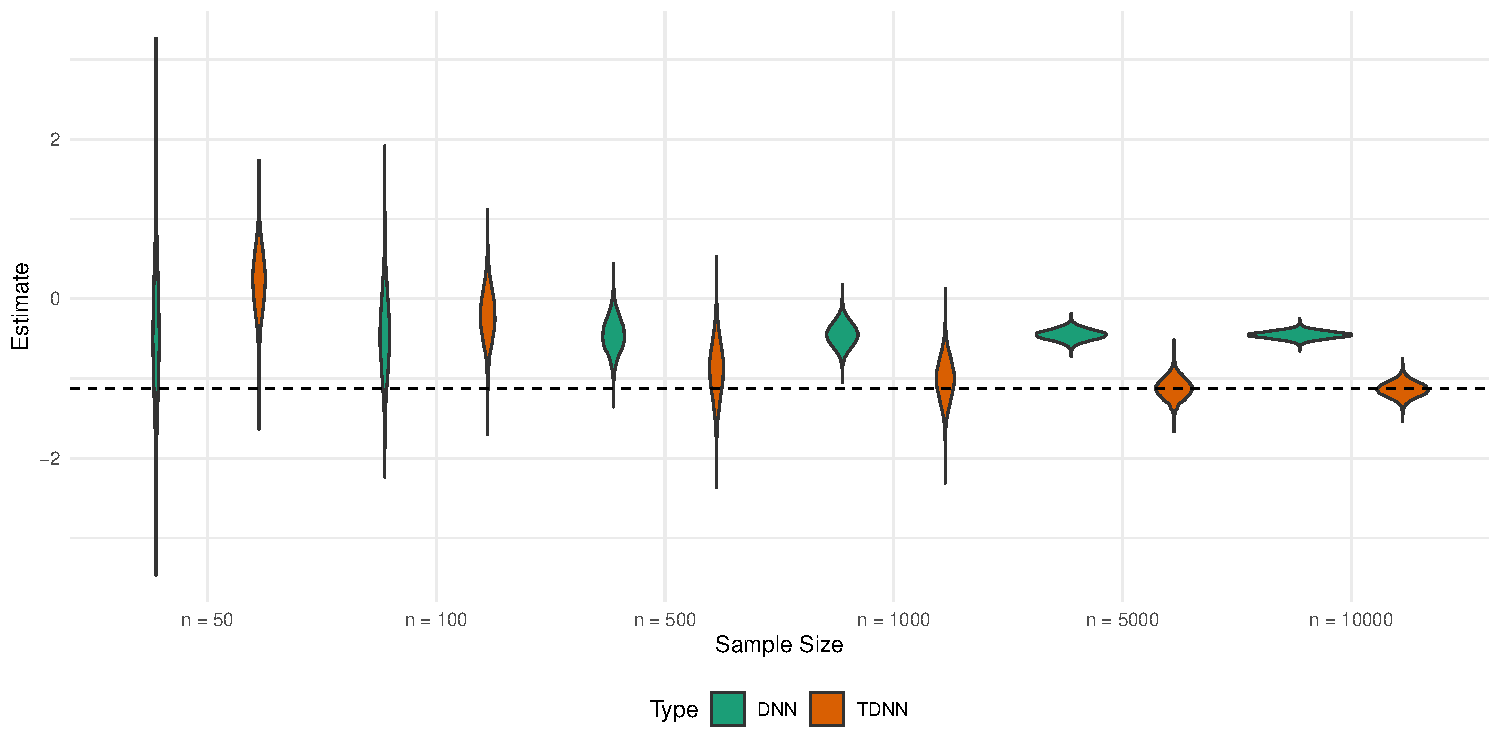
\includegraphics[width = \textwidth]{../Code/Simulations/Graphics/TDNN_DNN.pdf}
	\caption{Comparison of the DNN ($s = 20$) and TDNN ($s_1 = 20, s_2 = 50$) Estimators for different sample sizes.
		The dashed line indicates the value of the unknown regression function at the point of interest.
		Simulation Setup replicates Setting 1 from \citet{demirkaya_optimal_2024} for 10000 Monte Carlo Replications.}
\end{figure}

{\color{red} LOREM IPSUM}


\section{Application}\label{Application}
\hrule

\section{Conclusion}\label{Conclusion}
\hrule

\newpage
\printbibliography

\appendix
\section{Proofs}

% \section{PNN Calculations}
% \subsection{1-PNN Calculations}

% Due to the inherent connections between random forests and the \textit{Potential Nearest Neighbor} (PNN) framework, it is helpful to consider the properties of the k-PNN method first.
% Specifically, as we are considering large trees with a terminal node size of 1, we are interested in the properties of the 1-PNN framework.
% In this context, let $P_i(x)$ be an indicator for whether observation $i$ is a 1-PNN of a point of interest $x \in \mathbb{R}^d$.
% Furthermore, let $\operatorname{HR}(x,y)$ denote the hyperrectangle spanned by two points $x,y \in \mathbb{R}^d$ and by $x \prec y$ that $x \in \operatorname{HR}(\mathbf{0}, y)$ and by $x \not\prec y$ the complement of that event.

% Consider first the one-dimensional case and recall that given a subsample of indices $\mathcal{I}_S \subset \{1, \dotsc n\}$ with $i \in \mathcal{I}_S$ and $|\mathcal{I}_S| = s$, we have $P_i(x) = \mathbbm{1}(i = \argmin_{j \in \mathcal{I}_S} \|x - X_{j}\|)$.
% For simplicity and due to a symmetry of arguments, focus on the case of uniformly distributed features on $[0,1]$ and $x = 0$ and without loss of generality consider $i = 1$.
% This allows us to make the following observation
% \begin{equation*}
% 	\begin{aligned}
% 		\E\left[P_1 \, | \, Z_1\right]
% 		 & = \E\left[P_1 \, | \, X_1\right]
% 		= \P\left(X_1 = \min_{j \in \mathcal{I}_S} X_j \, | \, X_1\right)
% 		= \P(\forall j \in \mathcal{I}_S \backslash \{i\}: \, X_j > X_1 \, | \, X_1) \\
% 		 & = \P(B(s-1, X_1) = 0)
% 		= (1-X_1)^{s-1}.
% 	\end{aligned}
% \end{equation*}
% Similarly, consider the following, concentrating without loss of generality on $X_1$ and $X_2$ for $\{1,2\} \subset \mathcal{I}_S$ for $s \geq 2$.
% \begin{equation*}
% 	\begin{aligned}
% 		\E[P_1 \, | \, Z_1, Z_2]
% 		 & = \E[P_1 \, | \, X_1, X_2]
% 		= \P\left(X_1 = \min_{j \in \mathcal{I}_S} X_j \, \Big| \, X_1, X_2\right)                              \\
% 		 & = \P\left(X_1 = \min_{j \in \mathcal{I}_S} X_j \, \Big| \, X_1, X_2\right) \mathbbm{1}(X_1 \geq X_2)
% 		+ \P\left(X_1 = \min_{j \in \mathcal{I}_S} X_j \, \Big| \, X_1, X_2\right) \mathbbm{1}(X_1 < X_2)       \\
% 		% & = \P\left(X_1 = \min_{j \in \mathcal{I}_S} X_j \, \Big| \, X_1, X_2\right) \mathbbm{1}(X_1 \geq X_2)\\
% 		 & = \P\left(B(s-2, X_1) = 0\right) \mathbbm{1}(X_1 < X_2)
% 		= (1 - X_1)^{s-2} \mathbbm{1}(X_1 < X_2)                                                                \\
% 	\end{aligned}
% \end{equation*}
% Generalizing this idea, we can find that the following holds for the case of conditioning on $p \leq s $ observations, where wlog we consider $1, \dotsc, p \in \mathcal{I}_S$.
% \begin{equation*}
% 	\begin{aligned}
% 		\E[P_1 \, | \, Z_1, \dotsc, Z_p]
% 		 & = \E[P_1 \, | \, X_1, \dotsc, X_p]
% 		= (1 - X_1)^{s-p} \mathbbm{1}(\forall j = 2, \dotsc, p: \, X_1 < X_j).
% 	\end{aligned}
% \end{equation*}
% This is the first step to calculating the variances of the individual terms of the Hoeffding Decomposition of the weights for the 1-PNN method.
% Furthermore, we can recognize that the expectation of any sum of these conditional expectations has expectation equal to zero.
% For example, we can find the following
% \begin{equation*}
% 	\begin{aligned}
% 		\E\Bigl[\E[P_1 \, | \, Z_1, Z_2] - \E[P1 \, | \, Z_1]\Bigr]
% 		 & = \E\left[\E[P_1 \, | \, Z_1, Z_2]\right] - \E\left[\E[P1 \, | \, Z_1]\right]
% 		= \E\left[P_1\right] - \E\left[P_1\right]
% 		= 0.
% 	\end{aligned}
% \end{equation*}
% This, however, applies more broadly to sums of these terms, which is of interest in the upcoming calculations concerning the variances.
% Second, we need to consider the conditional expectations when conditioning on observations excluding i.
% As an illustrating example consider first the following
% \begin{equation*}
% 	\begin{aligned}
% 		\mathbb{E}[P_1 \, | \, Z_2]
% 		 & = \mathbb{E}[P_1 \, | \, X_2]
% 		= \mathbb{E}\left[\mathbb{E}[P_1 \, | \, X_1, X_2] \, | \, X_2\right]
% 		= \mathbb{E}\left[(1 - X_1)^{s-2} \mathbbm{1}(X_1 < X_2) \, | \, X_2\right] \\
% 		 & = \int_{0}^{X_2}(1 - x_1)^{s-2} \, dx_1
% 		% = -\frac{(1-X_2)^s - (1-X_2)}{(s-1)(1 - X_2)}
% 		= \frac{1 - (1-X_2)^{s-1}}{s-1}
% 	\end{aligned}
% \end{equation*}
% Similarly, we can consider conditioning on an arbitrary set of observations excluding $i=1$ and make use of the law of iterated expectations in an analogous manner.
% Without loss of generality, consider again $i = 1$ and conditioning on observations 2 to $p < s$ and to simplify the notation, let $\underline{X}_{2:p} = \min_{i = 2, \dotsc, p} X_i$.
% \begin{equation*}
% 	\begin{aligned}
% 		\mathbb{E}[P_1 \, | \, Z_2, \dotsc, Z_p]
% 		 & = \mathbb{E}[P_1 \, | \, X_2, \dotsc, X_p]
% 		= \mathbb{E}\left[\mathbb{E}\left[P_1 \, | \, X_1, X_2, \dotsc, X_p\right] \, | \, X_2, \dotsc, X_p\right] \\
% 		 & = \int_{0}^{\underline{X}_{2:p}}(1 - x_1)^{s-p} \, d x_1
% 		= \frac{1 - (1 - \underline{X}_{2:p})^{s+1-p}}{s + 1 - p}
% 	\end{aligned}
% \end{equation*}
% The next step is to consider the actual terms of the Hoeffding decomposition and evaluate their variance.
% First among them, we can find the following
% \begin{equation*}
% 	\begin{aligned}
% 		\Var(\E[P_1 \, | \, X_1])
% 		 & = \Var\left((1-X_1)^{s-1}\right)
% 		= \E\left[(1-X_1)^{2(s-1)}\right] - \E\left[(1-X_1)^{s-1}\right]^2                         \\
% 		 & = \int_{0}^{1} (1-x_1)^{2(s-1)} d x_1 - \left(\int_{0}^{1} (1-x_1)^{s-1} d x_1\right)^2
% 		= \frac{1}{2s - 1} - \frac{1}{s^2}                                                         \\
% 		 & \sim s^{-1}.
% 	\end{aligned}
% \end{equation*}
% To evaluate the variance of the second term, we can proceed by combining the expressions of the first and second conditional expectations.
% \begin{equation*}
% 	\begin{aligned}
% 		\E[P_1 \, | \, Z_1, Z_2] - \E[P1 \, | \, Z_1]
% 		 & = (1 - X_1)^{s-2} (\mathbbm{1}(X_1 < X_2) - (1 - X_1)) \\
% 		 & = (1 - X_1)^{s-2} (X_1 - \mathbbm{1}(X_1 \geq X_2)).
% 	\end{aligned}
% \end{equation*}
% Thus, to calculate the variance, observe that
% \begin{equation*}
% 	\begin{aligned}
% 		\Big|\E[P_1 \, | \, Z_1, Z_2] - \E[P_1 \, | \, Z_1]\Big|^2
% 		 & = \Big|(1 - X_1)^{s-2} (X_1 - \mathbbm{1}(X_1 \geq X_2)) \Big|^2            \\
% 		 & = (1 - X_1)^{2s-4}\Big|X_1 - \mathbbm{1}(X_1 \geq X_2) \Big|^2              \\
% 		 & = (1 - X_1)^{2s-4}\left(X_1^2 + \mathbbm{1}(X_1 \geq X_2)(1 - 2X_1)\right).
% 	\end{aligned}
% \end{equation*}
% and thus
% \begin{equation*}
% 	\begin{aligned}
% 		  & \Var(\E[P_1 \, | \, Z_1, Z_2] - \E[P1 \, | \, Z_1])
% 		= \E\left[(1 - X_1)^{2s-4}\left(X_1^2 + \mathbbm{1}(X_1 \geq X_2)(1 - 2X_1)\right)\right]                                                          \\
% 		= & \E\left[(1 - X_1)^{2s-4}X_1^2\right] + \E\left[(1 - X_1)^{2s-4}\mathbbm{1}(X_1 \geq X_2)(1 - 2X_1)\right]                                      \\
% 		= & \int_{0}^{1} (1 - x_1)^{2s-4}x_1^2 \, d x_1 + \int_{0}^{1}\int_{0}^{1}(1 - x_1)^{2s-4}\mathbbm{1}(x_1 \geq x_2)(1 - 2x_1) \, d x_1 \, d x_2    \\
% 		= & \int_{0}^{1} (1 - x_1)^{2s-4}x_1^2 \, d x_1 + \int_{0}^{1}\int_{x_2}^{1}(1 - x_1)^{2s-4}(1 - 2x_1) \, d x_1 \, d x_2                           \\
% 		= & \frac{1}{4s^3 - 12s^2 + 11s - 3} + \int_{0}^{1}\left[\frac{(1-x_2)^{2s-3}}{2s - 3}\left(1 - \frac{(2s - 3)x_2 + 1}{s-1}\right)\right] \, d x_2 \\
% 		= & \frac{1}{4s^3 - 12s^2 + 11s - 3} + \frac{5 - 2s}{-8s^3 + 24s^2 -22s + 6}
% 		\sim s^{-2}
% 	\end{aligned}
% \end{equation*}
% Furthermore, we can find that
% \begin{equation*}
% 	\begin{aligned}
% 		\operatorname{Var}\left(\mathbb{E}[P_1 \, | \, Z_2]\right)
% 		 & = \operatorname{Var}\left(\frac{1 - (1-X_2)^{s-1}}{s-1}\right)
% 		= \frac{1}{(s-1)^2} \operatorname{Var}\left((1-X_2)^{s-1}\right)                                                    \\
% 		 & = \frac{1}{(s-1)^2}\left(\mathbb{E}\left[(1-X_2)^{2(s-1)}\right] - \mathbb{E}\left[(1-X_2)^{s-1}\right]^2\right) \\
% 		 & = \frac{1}{(s-1)^2}\left(\frac{1}{2s - 1} - \frac{1}{s^2}\right)
% 		\sim s^{-3}
% 	\end{aligned}
% \end{equation*}
% This, in turn, implies the following
% \begin{equation*}
% 	\begin{aligned}
% 		\operatorname{Var}\left(\E[P_1 \, | \, Z_1, Z_2] - \E[P_1 \, | \, Z_1] + \E[P_2 \, | \, Z_1, Z_2] - \E[P_2 \, | \, Z_2]\right)
% 		\sim s^{-2}.
% 	\end{aligned}
% \end{equation*}

% To approach this problem more generally, it is imperative to find an expression for the variance of the c'th term of the Hoeffding decomposition.
% Now, fixing $P_1$ as the weight of interest, recall in analogy to the beginning of this paper the following term:
% \begin{equation*}
% 	A_1^{(k)}
% 	:= \sum_{E \in P_{s,k-1}^{\{1\}}} \left(-1\right)^{\mathbbm{1}\left(|E| \equiv (k-1) \mod 2\right)} \mathbb{E}\left[P_1 \, | \, X_1, X_e \, : \, e \in E\right].
% \end{equation*}
% As this term forms the core of the kernel of the relevant Hoeffding decomposition, it will allow us to gain a better understanding of the relevant variances at play.
% First, by a simple application of the law of iterated expectations, we find that $\mathbb{E}[A_1^{(k)}] = 0$.
% Thus, to understand its variance, we need to investigate $\mathbb{E}\left[|A_1^{(k)}|^2\right]$.
% \begin{equation*}
% 	\begin{aligned}
% 		|A_1^{(k)}|^2
% 		 & = \sum_{E, E' \in P_{s,k-1}^{\{1\}}}
% 		(-1)^{\mathbbm{1}(|E| + | E'| \equiv 0 \mod 2)}
% 		\left\{\mathbb{E}\left[P_1 \, | \, X_1, X_e \, : \, e \in E\right] \mathbb{E}\left[P_1 \, | \, X_1, X_{e'} \, : \, e' \in E'\right]\right\}
% 	\end{aligned}
% \end{equation*}
% As this expression shows, we are interested in expressions of the following form
% \begin{equation*}
% 	\begin{aligned}
% 		\mathbb{E}\Bigl[\mathbb{E}\left[P_1 \, | \, X_1, X_e \, : \, e \in E\right] \mathbb{E}\left[P_1 \, | \, X_1, X_{e'} \, : \, e' \in E'\right]\Bigr]
% 	\end{aligned}
% \end{equation*}
% Now, fix $E, E' \in P_{s,k-1}^{\{1\}}$, and let $F = E \cap E'$.
% Given this now fixed expression, we can continue our analysis in the following way.
% \begin{equation*}
% 	\begin{aligned}
% 		A_{E, E'}
% 		:= & \mathbb{E}\Bigl[\mathbb{E}\left[P_1 \, | \, X_1, X_e \, : \, e \in E\right] \mathbb{E}\left[P_1 \, | \, X_1, X_{e'} \, : \, e' \in E'\right]\Bigr]        \\
% 		=  & \mathbb{E}\left[(1 - X_1)^{s-|E|-1} \mathbbm{1}(\forall j \in E: \, X_1 < X_j) \, (1 - X_1)^{s-|E'|-1} \mathbbm{1}(\forall j \in E': \, X_1 < X_j)\right] \\
% 		=  & \mathbb{E}\left[(1-X_1)^{2s - |E| - |E'| - 2}\mathbbm{1}(\forall j \in E \cup E': \, X_1 < X_j)\right]                                                    \\
% 		=  & \mathbb{E}\left[(1-X_1)^{2s - \mathcal{E} - \mathcal{E}' - 2}\mathbbm{1}(\forall j \in E \cup E': \, X_1 < X_j)\right]
% 	\end{aligned}
% \end{equation*}
% Here, to simplify the notation, we let $\mathcal{E} = |E|,$ $\mathcal{E}' = |E'|$ and $\mathcal{F} = |F|$.
% Recall that we are dealing with independent and identically uniformly distributed features, such that we can simplify this expectation by considering the density of the minimum of $\mathfrak{E} = \mathcal{E} + \mathcal{E}' - \mathcal{F}$ i.i.d. uniform random variables instead of the multivariate integral.
% Specifically, realize that defining $W = \min_{e \in E \cup E'} X_e$, $W$ is distributed according to the following density function.
% \begin{equation*}
% 	\begin{aligned}
% 		f_W(w) = \begin{cases}
% 			         \mathfrak{E}\left(1-w\right)^{\mathfrak{E}- 1} & \text{if } w \in [0,1] \\
% 			         0                                              & \text{otherwise}
% 		         \end{cases}.
% 	\end{aligned}
% \end{equation*}
% Using this expression, we find that
% \begin{equation*}
% 	\begin{aligned}
% 		A_{E, E'}
% 		 & = \int_{0}^{1}\left(\mathfrak{E}\left(1-w\right)^{\mathfrak{E}- 1}\int_{0}^{w} (1-x_1)^{2s - \mathcal{E} - \mathcal{E}' - 2} \, dx_1 \right) \, dw                                                     \\
% 		 & = \int_{0}^{1}\left(\mathfrak{E}\left(1-w\right)^{\mathfrak{E}- 1} \frac{1}{2s - \mathcal{E} - \mathcal{E}' - 1}\left(1 - \left(1 - w\right)^{2s - \mathcal{E} - \mathcal{E}' - 1}\right)\right) \, dw \\
% 		 & =  \frac{1}{2s - \mathcal{E} - \mathcal{E}' - 1}\left(1 -\int_{0}^{1} \mathfrak{E}\left(1-w\right)^{\mathfrak{E}- 1}\left(1 - w\right)^{2s - \mathcal{E} - \mathcal{E}' - 1} \, dw\right)              \\
% 		 & =  \frac{1}{2s - \mathfrak{E} + \mathcal{F} - 1}\left(1 - \mathfrak{E}\int_{0}^{1} \left(1 - w\right)^{2s - \mathcal{F} - 2} \, dw\right)                                                              \\
% 		 & = \frac{1}{2s - \mathfrak{E} + \mathcal{F} - 1}\left(1 - \frac{\mathfrak{E}}{2s - \mathcal{F} - 1}\right)
% 		= \frac{2s -\mathfrak{E} - \mathcal{F} - 1 }{2s - \mathfrak{E} + \mathcal{F} - 1}\left(2s - \mathcal{F} - 1\right)^{-1}                                                                                   \\
% 		 & \sim s^{-1}
% 	\end{aligned}
% \end{equation*}
% Considering this notation, we can write the expression of interest in the following way to continue investigating its behavior.
% \begin{equation*}
% 	\begin{aligned}
% 		|A_1^{(k)}|^2
% 		= \sum_{E, E' \in P_{s,k-1}^{\{1\}}}(-1)^{\mathbbm{1}(|E| + | E'| \equiv 0 \mod 2)}A_{E, E'}
% 	\end{aligned}
% \end{equation*}

% Considering the original test case of $k = 2$, we can check whether this approach gives us the same results.
% \begin{equation*}
% 	\begin{aligned}
% 		|A_1^{(2)}|^2
% 		 & = \sum_{E, E' \in P_{s,1}^{\{1\}}} (-1)^{\mathbbm{1}(|E| + | E'| \equiv 0 \mod 2)}A_{E, E'}                                        \\
% 		 & = (s-1)A_{\{2\},\{2\}} + (s-1)(s-2)A_{\{2\},\{3\}} - 2(s-1)A_{\{2\}, \emptyset} + A_{\emptyset, \emptyset}                         \\
% 		 & = \frac{(s-1)(2s - 4)}{(2s - 2)(2s - 2)} + \frac{(s-1)(s-2)(2s - 3)}{(2s - 1)(2s - 1)} - \frac{2(s-1)(2s - 2)}{(2s - 2)(2s - 1)} + \\
% 		 & = \frac{s - 2}{2s - 2} + \frac{(s-1)(s-2)(2s - 3)}{(2s - 1)(2s - 1)} - \frac{2(s-1)}{2s - 1}                                       \\
% 	\end{aligned}
% \end{equation*}
% {\color{red} LOREM IPSUM! I found a mistake. Will fix soon.}

% Thus, recall the following recursive Kernel definition that forms the basis to the Hoeffding decomposition.
% \begin{align*}
% 	h^{(1)}(x_1)
% 	 & = \psi_1(x_1) - \theta                                                                                \\
% 	h^{(c)}(x_1, x_2, \dotsc, x_c)
% 	 & = \psi_c(x_1, \dotsc, x_c) - \sum_{j = 1}^{c-1}\sum_{(c,j)}h^{(j)}(x_{i_1}, \dotsc, x_{i_j}) - \theta
% \end{align*}
% To illustrate the connection to the problem at hand, fix first $P_1$ as the weight of interest.
% Then, in an abuse of notation, consider $\psi_c(x_{i_1}, \dotsc, x_{i_j}) = \mathbb{E}\left[P_1 \, | \, X_{i_1} = x_{i_1}, \dotsc, X_{i_j} = x_{i_j}\right]$.

% \subsection{1-PNN in d Dimensions}

% Next, consider the case of uniformly distributed features on $[0,1]^d$ with the point of interest at the origin, i.e. $x = \mathbf{0}$.
% Similar to the one-dimensional case, the argument will extend to other points under consideration and other suitable distributions.

% What this choice allows us to do is consider a simplified form of the probability of a point being a 1-PNN.
% Thus, observe that the probability of a sample point $X_1$ being a 1-PNN of the origin, i.e. the expectation of $P_1$, can be expressed in the following form
% \begin{equation*}
% 	\begin{aligned}
% 		\mathbb{E}[P_1 \, | \, X_1]
% 		 & = \mathbb{P}(X_1 \text{ is a 1-PNN of } \mathbf{0} \, | \, X_1)                                            \\
% 		 & = \mathbb{P}\left(\bigcap_{j = 2}^{s} \{X_j \not\in \operatorname{HR}(\mathbf{0}, X_1)\, | \, X_1\}\right)
% 		= \mathbb{P}\left(\bigcap_{j = 2}^{s}\bigcap_{k = 1}^{d} \{X_{jk} \not\in [0, X_{1,k}]\, | \, X_1\}\right)    \\
% 		 & = \mathbb{P}\left(B\left(s - 1, \prod_{k = 1}^{d} X_{1,k}\right) = 0\, | \, X_1\right)
% 		= \mathbb{P}\left(B\left(s - 1, X_{1, \bullet}\right) = 0\, | \, X_1\right)                                   \\
% 		 & = (1-X_{1, \bullet})^{s-1},
% 	\end{aligned}
% \end{equation*}
% where we let $X_{i,\bullet}$ denote $\prod_{k = 1}^{d} X_{i,k}$.
% To calculate the variance of the conditional expectation, consider the following rewriting
% \begin{equation*}
% 	\begin{aligned}
% 		\operatorname{Var}\left(\mathbb{E}[P_1 \, | \, X_1]\right)
% 		% & = \operatorname{Var}\left((1-X_{1, \bullet})^{s-1}\right) 
% 		 & = \mathbb{E}[(1-X_{1, \bullet})^{2(s-1)}] - \left(\mathbb{E}[(1-X_{1, \bullet})^{s-1}]\right)^2.
% 	\end{aligned}
% \end{equation*}
% Now, notice that $X_{1,\bullet}$ is distributed according to the density
% \begin{equation*}
% 	f_{1, \bullet}(x) = \begin{cases}
% 		\frac{(-\log{(x)})^{d-1}}{(d-1)!} & \text{for } 0\leq x \leq 1 \\
% 		0                                 & \text{otherwise}
% 	\end{cases}.
% \end{equation*}
% Using this density, we can solve for the variance in the following way
% \begin{equation*}
% 	\begin{aligned}
% 		\operatorname{Var}\left(\mathbb{E}[P_1 \, | \, X_1]\right)
% 		 & = \int_{0}^{1} \frac{(-\log{(x)})^{d-1}}{(d-1)!} (1-x)^{2(s-1)} \, dx - \left(\int_{0}^{1} \frac{(-\log{(x)})^{d-1}}{(d-1)!}(1-x)^{s-1} \, dx\right)^2 \\
% 		 & = {\color{red}\text{Tedious... but needs a good argument}}                                                                                             \\
% 		 & \sim s^{-1} \quad {\color{red} \text{I assume...}}
% 	\end{aligned}
% \end{equation*}

% Proceeding as in the one-dimensional case, we consider next the conditional expectation of $P_1$ given $Z_1$ and $Z_2$, where these choices are again without loss of generality.
% \begin{equation*}
% 	\begin{aligned}
% 		\mathbb{E}[P_1 \, | \, Z_1, Z_2]
% 		 & = \mathbb{E}[P_1 \, | \, X_1, X_2]
% 		= \mathbbm{1}_{(X_2 \prec X_1)}\mathbb{E}[P_1 \, | \, X_1, X_2, X_2 \prec X_1] + \mathbbm{1}_{(X_2 \not\prec X_1)}\mathbb{E}[P_1 \, | \, X_1, X_2, X_2 \not\prec X_1] \\
% 		 & = \mathbbm{1}_{(X_2 \not\prec X_1)}\mathbb{E}[P_1 \, | \, X_1, X_2, X_2 \not\prec X_1]
% 		= \mathbbm{1}_{(X_2 \not\prec X_1)} \mathbb{P}\left(B\left(s - 2, \prod_{k = 1}^{d} X_{1,k}\right) = 0\, | \, X_1\right)                                              \\
% 		 & = \mathbbm{1}_{(X_2 \not\prec X_1)} (1- X_{1,\bullet})^{s-2}.
% 	\end{aligned}
% \end{equation*}
% {\color{red} LOREM IPSUM}


\end{document}

% \citet{peng_rates_2022}
% {\color{red} Combine Theorem 1 and a variation of the argument for Proposition 1 to improve rate for point-wise inference.
% 	Better rate of subsampling scale with sample size.}

% \vspace{0.5cm}
% \begin{theorem}[Theorem 1 - \citet{peng_rates_2022}]\label{PengThm1}
% 	Let $\mathbf{Z}_1, \ldots, \mathbf{Z}_n$ be i.i.d. from $P$ and $U_{n, s, \omega}$ be a generalized complete $U$-statistic with kernel $h\left(\mathbf{Z}_1, \ldots, \mathbf{Z}_s ; \omega\right)$.
% 	Let $\theta=\mathbb{E}[h], \zeta_{1, \omega}=\operatorname{Var}\left(\mathbb{E}\left[h \mid Z_1\right]\right)$ and $\zeta_s=\operatorname{var}(h)$.

% 	If $\frac{s}{n} \frac{\zeta_s}{s \zeta_{1, \omega}} \rightarrow 0$, then
% 	\begin{equation}
% 		\frac{U_{n, s, \omega}-\theta}{\sqrt{s^2 \zeta_{1, \omega} / n}} \rightsquigarrow N(0,1) .
% 	\end{equation}
% \end{theorem}
% In a remark to this Theorem, the authors state that when the variance ratio $\frac{\zeta_s}{s\zeta_{1,\omega}}$ is bounded, choosing $s = o(n)$ is sufficient to ensure that Theorem \ref{PengThm1} applies.
% A more directly applicable result comes from Proposition 2 of the same paper.

% \vspace{0.5cm}
% \begin{theorem}[Proposition 2 - \citet{peng_rates_2022}]
% 	Let $\mathbf{Z}_1, \ldots, \mathbf{Z}_s$ denote i.i.d. pairs of random variables $\left(\mathbf{X}_i, Y_i\right)$.
% 	Suppose $Y_i=\mu\left(X_i\right)+\varepsilon_i$ where $\mu$ is bounded, $\varepsilon$ has mean 0 and variance $\sigma^2$, and $\mathbf{X}_i$ and $\varepsilon_i$ are independent.
% 	Let $\varphi=\sum_{i=1}^s w(\mathbf{x}, \mathbf{X}_i, \mathfrak{X}) Y_i$ such that $\sum_{i=1}^s w(\mathbf{x}, \mathbf{X}_i, \mathfrak{X})=1$, where $\mathfrak{X}$ denotes $\left\{X_i\right\}_{i=1}^m$.
% 	Then
% 	\begin{equation}
% 		\limsup _{s \rightarrow \infty} \frac{\zeta_s}{s^2 \zeta_1}
% 		< \infty.
% 	\end{equation}
% \end{theorem}

% Following from the representation of the WNN estimator as an L-statistic in \citet{steele_exact_2009}, both the DNN and TDNN estimators are of this form.
% Thus, we can deduce the following.
% \begin{equation}
% 	\limsup _{s \rightarrow \infty} \frac{1}{s^2} \frac{\operatorname{Var}\left(h_{s}\left(\mathbf{x}; D_{\ell}\right)\right)}{\operatorname{Cov}\left(h_s\left(\mathbf{x}; D_{\ell}\right), h_s\left(\mathbf{x}; D_{\ell'}\right)\right)}
% 	< \infty
% \end{equation}
% where $D_{\ell}$ and $D_{\ell'}$ only share exactly one observation, say $\mathbf{Z}_1$.